\section{Illustration}
\label{sec:illust}

\newcommand{\allp}{\texttt{all\_p}}
\newcommand{\onp}{\texttt{on\_p}}
\newcommand{\offp}{\texttt{off\_p}}
\newcommand{\hystp}{\texttt{hyst\_p}}
\newcommand{\aonebelow}{\texttt{a1\_below}}
\newcommand{\atwobelow}{\texttt{a2\_below}}
\newcommand{\aoneabove}{\texttt{a1\_above}}
\newcommand{\atwoabove}{\texttt{a2\_above}}
\newcommand{\doion}{\texttt{doi\_on}}
\newcommand{\done}{\texttt{d1}}
\newcommand{\dtwo}{\texttt{d2}}
\newcommand{\abovehyst}{\texttt{above\_hyst}}
\newcommand{\inhibit}{\texttt{inhibit}}

We illustrate the idea of completeness metrics and the ``score" from different metrics on our altitude switch (ASW) example from Section~\ref{sec:example}.  %In so doing, we hope to motivate the need for completeness metrics and also to justify our proof-based approaches.
%
The ASW is responsible for turning on and off a device of interest, so we formulate two requirements that describe when the ASW should be {\em on} and when it should be {\em off}.  We illustrate the results with traceability matrices produced by the Spear tool~\cite{Spear}, which is discussed in Section~\ref{sec:impl}.

The first attempt at formalization (property set 1) is as follows:

%\begin{definition} {\emph{ASW Requirements Version 1} }
{\smaller
\begin{verbatim}
on_p = (a1_below and a2_below) and not inhibit =>
    doi_on = true;
off_p = (a1_above and a2_above) and inhibit =>
    doi_on = false;
all_p = on_p and off_p;
\end{verbatim}
}
%\end{definition}

\begin{figure}
  \centering
  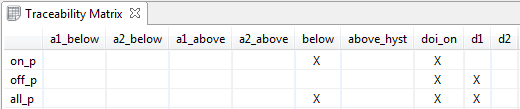
\includegraphics[width=0.9\columnwidth]{figs/spear_set1.png}
  \vspace{-0.1in}
  \caption{Elements covered by the initial property set}
  \vspace{-0.1in}
  \label{fig:propertyset1}
\end{figure}


\noindent Informally, when both altimeters are below the threshold and not inhibited, then the DOI should be on ({\small \onp}), and when both altimeters are below the threshold and the ASW is inhibited, then the DOI should be off ({\small \offp}).
For each of the \ivccov, \maycov, and \mustcov\ metrics, {\small \allp} ~only requires {\small \texttt{\{below, d1, doi\_on\}}}, as shown in Figure~\ref{fig:propertyset1}.
This small set of elements is due to a classic specification problem: using computed variables as the antecedents of implications.  If these values are computed incorrectly (say, we choose the wrong threshold for {\small \aonebelow }), it may cause the property to be valid for incorrect reasons.

%This is alarming, and somewhat puzzling, because one would think that at least the definitions of the `below' or `above' would be necessary.  However, because the specification used the model variables \aonebelow, \atwobelow, \aoneabove, and \atwoabove, the actual valuations of the thresholds do not matter.  This situation illustrates a classic specification problem: using computed variables in the antecedents of implications.
%\footnote{\noindent ~In this case, if the computation of the variables used in the antecedent is incorrect, then our property will not verify what it is expected to verify \mike{citation to one of our papers on specification here...}; note also that this does not mean the property is necessarily {\em vacuous}.}

We therefore modify our properties to use inputs and constants as antecedents and derive:

{\smaller
\begin{verbatim}
on_p = ((alt1 < THRESHOLD) and (alt2 < THRESHOLD))
   and not inhibit => doi_on = true;
off_p = ((alt1 >= T_HYST) and (alt2 >= T_HYST))
   and inhibit => doi_on = false;
\end{verbatim}
}
% all_p = on_p and off_p;
%\end{definition}

\noindent In this version, distinctions emerge between the metrics.  {\small \allp } ~has two \mivc s: {\small{ \texttt{\{\{a1\_below, below, doi\_on, d1\}, \{a2\_below, below, doi\_on, d1\}\}}}}, 
because of the {\small { \onp }} ~property: in the implementation, the DOI is turned on when either of the altimeters is below the threshold, while our property states that they both must be below.
Domain experts determine that the requirement is correctly specified and that our implementation is a reasonable refinement, so there is no need to change the model or the property.  The MUST elements are the same as version 1: {\small{ \texttt{\{below, doi\_on, d1\}}}}, because neither {\small \aonebelow }~ or {\small {\atwobelow}} ~is required for all proofs.  %However, given the MUST elements, we can no longer construct a proof, because at one of these definitions is necessary for either proof.
The MAY elements contain both {\small \aonebelow } ~and {\small \atwobelow }.

The {\small { \abovehyst, \aoneabove, \atwoabove,} } and {\small{ \dtwo }} ~equations are still missing, meaning that the ``above'' thresholds are irrelevant to our properties.  Examining {\small \offp }, we realize that we have a specification error; the DOI should be off if either  {\small \inhibit }
~is true or both altimeters are above the threshold. The fix is:

%\begin{definition} {\emph{ASW Requirements Version 2} }
{\smaller
\begin{verbatim}
off_p = ((alt1 >= T_HYST) and (alt2 >= T_HYST))
   or inhibit => doi_on = false;
\end{verbatim}
}
%on_p = ((alt1 < THRESHOLD) and (alt2 < THRESHOLD))
%   and not inhibit => doi_on = true;
%all_p = on_p and off_p;
%\end{definition}

\noindent Now the {\small{ \allp}} ~requirement proof yields a single \mivc ~that requires all variables except {\small{ \{\texttt{d2}\}}}, so \mivc ~= MAY = MUST.  Interestingly, the {\small{\offp}} ~proof requires both the lower altimeter thresholds even though the {\small{ \onp}} ~proof does not; the reason is that if either of these is false, then {\small{ \doion}} ~will be true.  To cover {\small{ \{\texttt{d2}\}}}, we realize no property covers the hysteresis case, so an additional property is added for this case:

%\begin{definition} {\emph{ASW Requirements Version 2} }
{\smaller
\begin{verbatim}
hyst_p = not inhibit and
         (alt1 > THRESHOLD and alt2 > THRESHOLD) and
         (alt1 < T_HYST or alt2 < T_HYST) =>
   (doi_on = false -> doi_on = pre(doi_on))
all_p = on_p and off_p and hyst_p;
\end{verbatim}
}
%on_p = ((alt1 < THRESHOLD) and (alt2 < THRESHOLD))
%   and not inhibit => doi_on = true;
%all_p = on_p and off_p;
%\end{definition}
\noindent The final property states that if the antecedent conditions hold, then in the initial state, the {\small{\doion}} variable is assigned false, and in subsequent steps, it retains the same value as it previously had.

\begin{figure}
  \centering
  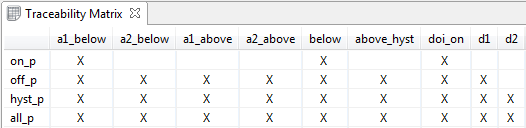
\includegraphics[width=0.9\columnwidth]{figs/spear_set4.png}
  \vspace{-0.1in}
  \caption{Elements covered by the final property set}
  \vspace{-0.1in}
  \label{fig:propertyset4}
\end{figure}

As shown in Figure~\ref{fig:propertyset4}, the measures again coincide and include all variables, and we appear to have a reasonably complete specification.  However, the measures are certainly not foolproof; it turns out that using {\em only} the hysteresis property {\small{ \hystp}} ~will {\em also} yield a ``complete'' result for all of the metrics: to establish its validity, all of the equations that we have defined in the model are required.  This is because the partitioning of the transition system (i.e., the equations) is insufficiently {\em granular} to detect the incompleteness.
%However, this one property would not reasonably be considered a complete specification.
We will examine this situation further in Section~\ref{sec:discussion}.
%We will examine this situation further in the discussion section~\mike{add this!}.
%
%\mike{How would we define a metric that would flag the model as incomplete?  Model transformation would do it: if we added separate variables for each assignment of doi\_on, then any of the metrics would flag the \hystp\ spec as incomplete.}
